\chapter{Experimental Setup: Design, Integration, and Evaluation Metrics}
\label{chapter:test-bench-design}

This chapter describes the design of the complete system test setup developed for radiation testing of the motor controller. The objective was to build an easily reproducible test bench that minimizes the overhead involved in replacing irradiated parts, updating firmware, or reconfiguring the data acquisition system between test campaigns. It covers the mechanical design for PCB, magnet, motor, and resolver integration, the data acquisition software, and the methodology used to process and evaluate the resulting test data.

\section{System Requirements and Constraints}
\label{sec:system-requirements}

This section outlines the functional integration requirements and the constraints imposed by the irradiation facilities.

\subsection{Evaluation Methodology}
\label{subsec:evaluation-methodology}
The motor controller is evaluated in position control mode for two main reasons. First, robotic arm applications are inherently servo applications, making position accuracy the most relevant performance metric. Second, resolver-based position readout is more reliable than velocity estimation, as sampling the angle at regular intervals avoids the information loss introduced by numerical differentiation between samples.

\subsection{Resolver and Readout System}
\label{subsec:resolver-readout}

The resolver integrated in this setup is the same model used in the collimator stepper motor systems of the accelerators, where it is actively maintained and operated by the BE-CEM-MRO section. This choice ensures compatibility with existing infrastructure and validated readout electronics.

For reading the resolver output, the \textit{EVAL-AS2S1210} evaluation board by Analog Devices is used, which is based on the same IC used by BE-CEM-MRO in their collimator systems. The resolver requires its signal cables to be routed as twisted pairs to maintain signal integrity, which has direct consequences on the cabling strategy described in Section~\ref{subsec:resolver-cabling}.

A custom BE-CEM-MRO readout solution for the \texttt{AS2S1210} has been developed to eliminate reliance on the vendor's proprietary software. The custom solution makes use of the \texttt{EVAL-AS2S1210} paired with a Raspberry Pi, which serves as a serial to SPI driver~\cite{weber2026rpfirmware}. This straightforward setup enables resolver readout through simple serial commands issued from either Python or C++ code.

\subsection{Irradiation Facility Constraints}
\label{subsec:facility-constraints}
The setup must be compatible with three irradiation facilities: i) CHARM, ii) PSI PIF, and iii) CC60. While these facilities differ in beam type and geometry, the most relevant parameters for setup design are the radiation environment and the available cabling infrastructure.

In CC60 and PSI PIF, only a localised region around the device under test is irradiated, so sensitive supporting equipment can be placed at a safe distance. In CHARM, however, the entire room is irradiated. Therefore, equipment such as UART-to-USB converters and the resolver readout board must be located outside the irradiation room in all cases to ensure compatibility across all three facilities.

All three facilities share a similar cabling infrastructure, with patch panels supporting BNC, RJ45, and USB connectors. For this setup, BNC and RJ45 connectors are used. RJ45 is particularly well suited for resolver signal routing, as standard Ethernet cables contain twisted pairs that directly satisfy the resolver's signal integrity requirements without additional specialised cabling. The resulting connectivity is illustrated in Figure~\ref{fig:irradiation-control-rooms}.

\begin{figure}[H]
\centering
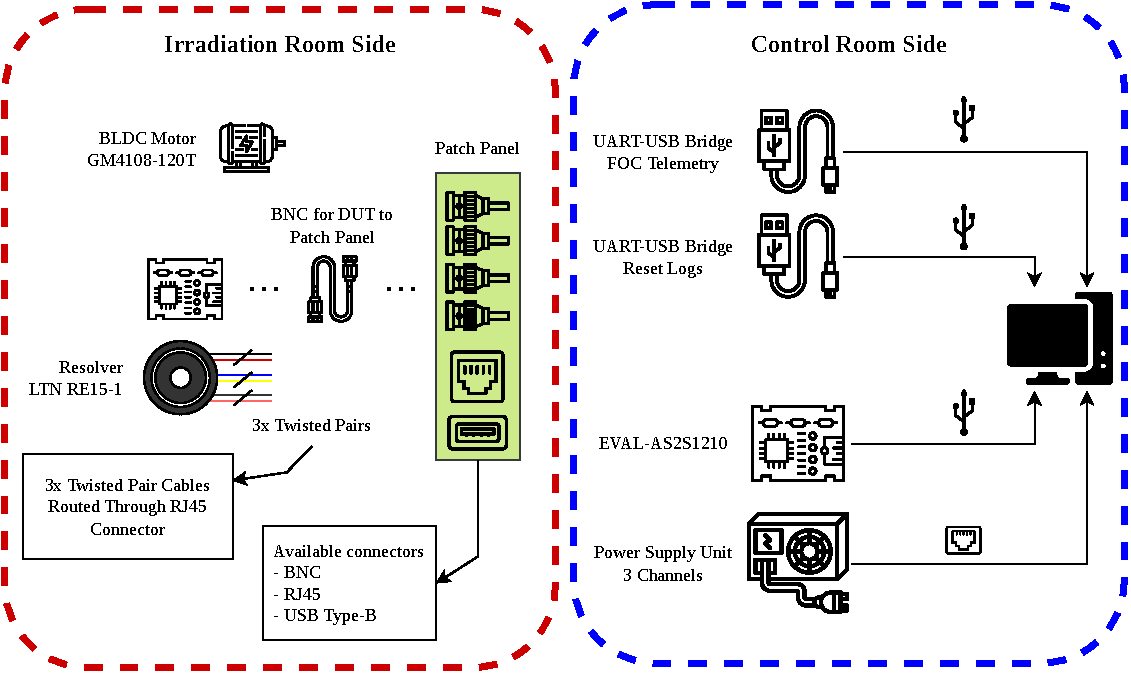
\includegraphics[width=\textwidth, keepaspectratio]{05_SystemLevelTestBench/images/Irradiation_Control_Rooms.pdf}
\caption{Signal routing between the irradiation room and the control room, showing the connector infrastructure used across facilities.}
\label{fig:irradiation-control-rooms}
\end{figure}

\section{Mechanical Design of the Test Bench}
\label{sec:cad-test-bench-design}

The mechanical structure integrating all system components was designed in SOLIDWORKS. Since the motor used in this setup has a hollow shaft, the design is governed by strict alignment requirements, as the accuracy of the system depends on the correct positioning of each component along a common axis passing through it:

\begin{itemize}
\item The permanent magnet must be fixed at the center of the rotor and aligned to the magnetic encoder with a maximum axial offset of 1\,mm.
\item The resolver rotor must be co-axial with the motor rotor and free to spin without any contact with the resolver stator.
\end{itemize}

\subsection{Test Bench Structure Design}

The design was done using SOLIDWORKS and revolves around aligning the components in the same axis. In the following figure \ref{fig:assembly-panoramic} an overview of the system is showcased. The mechanical structure is mounted on the PCB at 4 different points and connected to the common ground. Inside the "box" with the black color is the representation of the PMSM and on the top the green ring is the resolver stator and the brown ring is its rotor. From a functional point of view, the rotor of the resolver is attached to the motors' rotor by using a washer and an M5 screw. This will become clearer in the following figures though.

\begin{figure}[H]
    \centering
    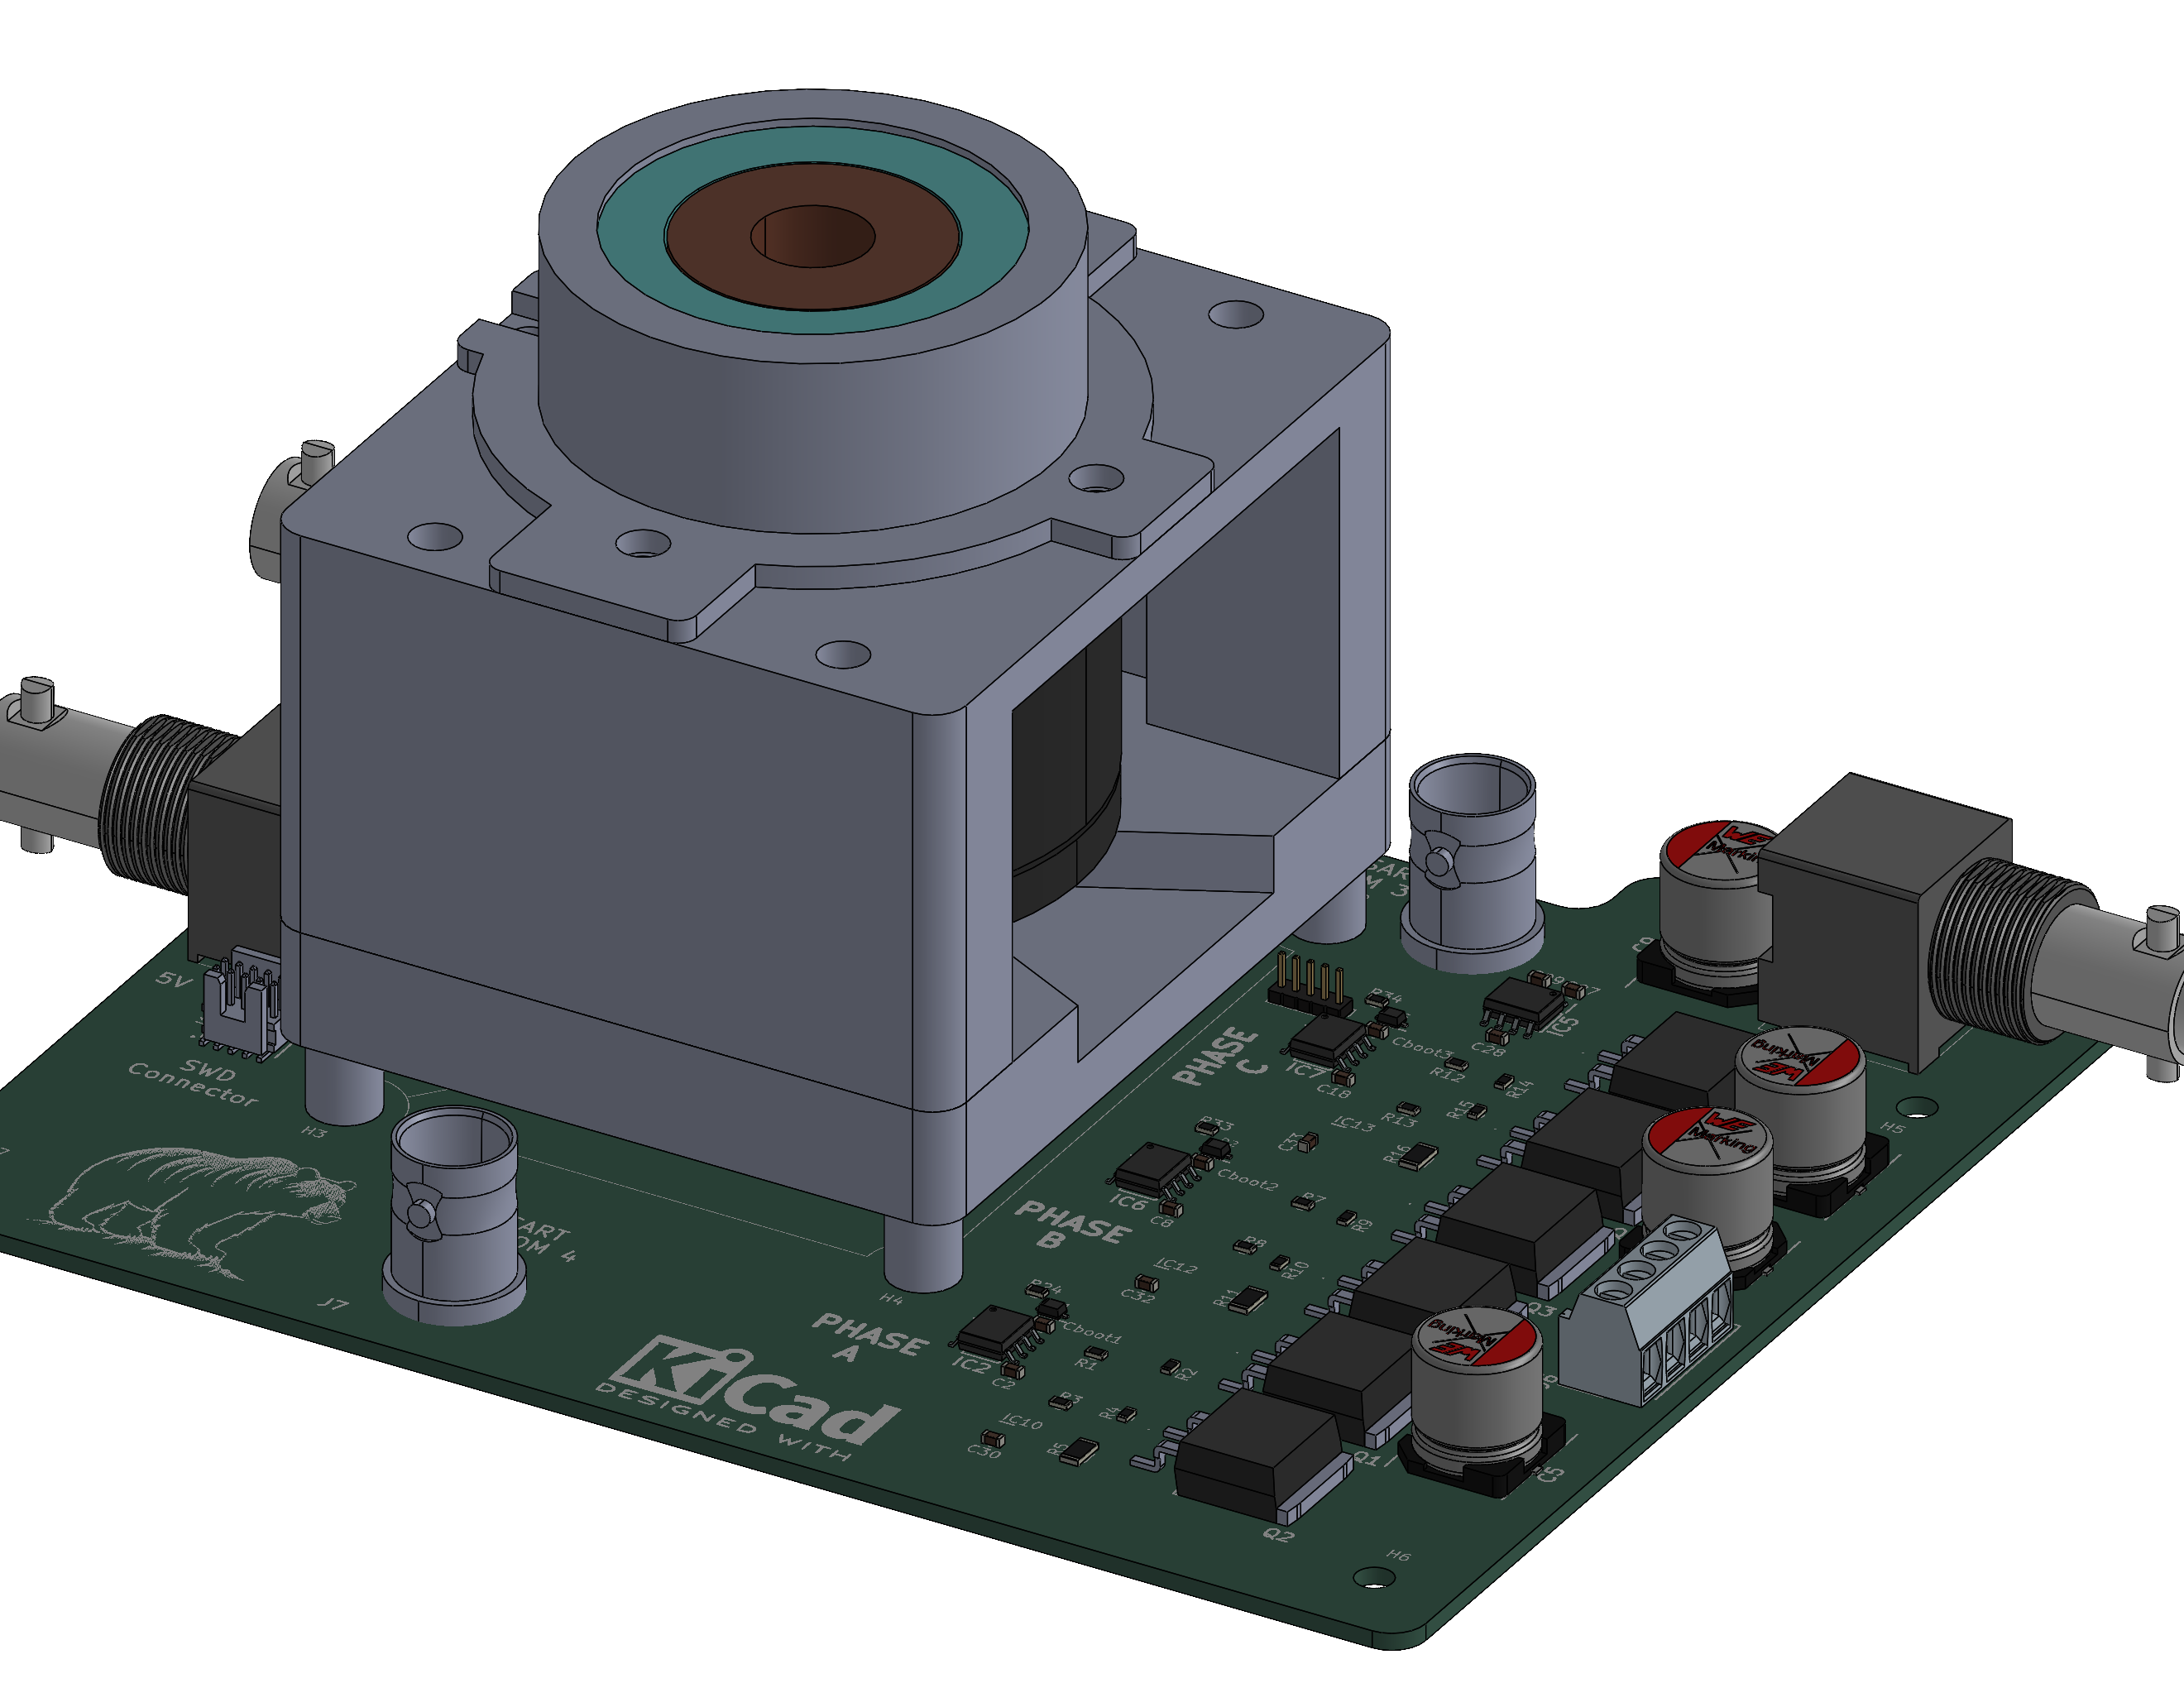
\includegraphics[width=0.6\textwidth, keepaspectratio]{05_SystemLevelTestBench/images/Resolver-PCB-Setup-1.PNG}
    \caption{3D view of the complete mechanical assembly and the PCB of the second iteration system [\ref{subsec:pcb-iter-2}]}
    \label{fig:assembly-panoramic}
\end{figure}

The last missing part of the alignment is to make clear how the magnet is aligned on z-axis and xy-plane to the magnetic encoder. In the following figure \ref{fig:assembly-magnet-alignment} the attempt is to show exactly this

\begin{figure}[H]
    \centering

    \begin{subfigure}[b]{0.48\textwidth}
        \centering
        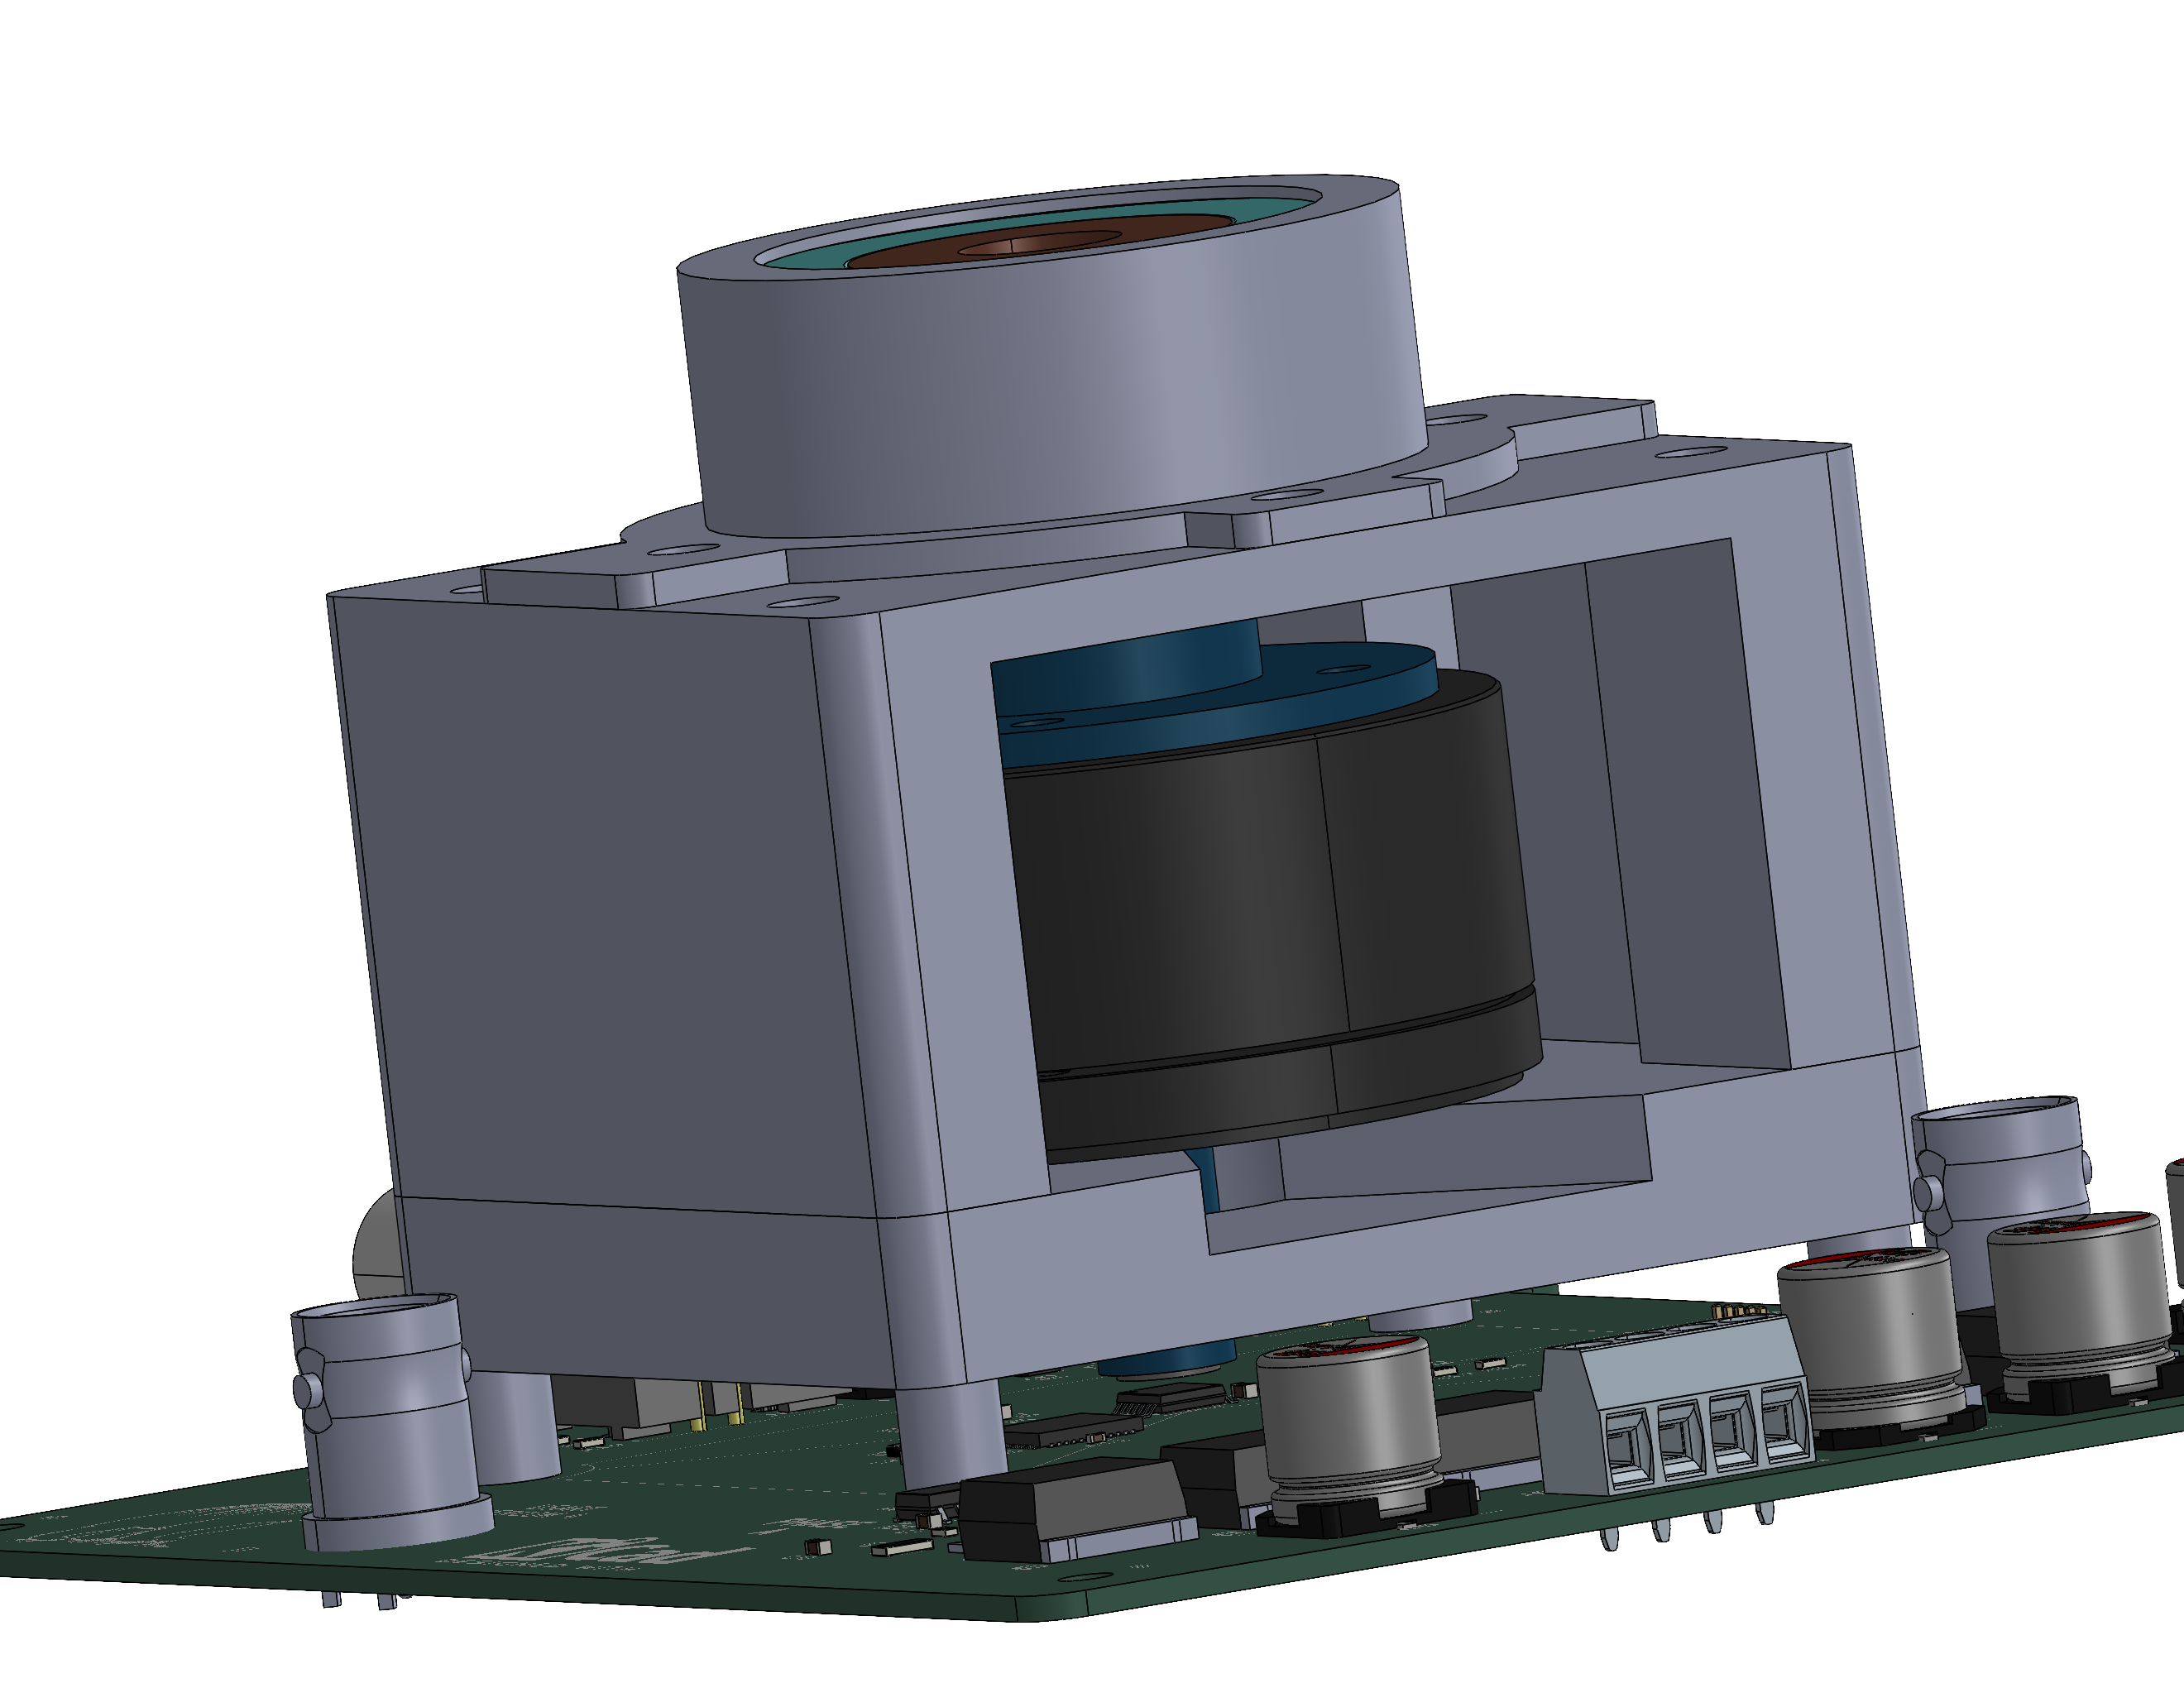
\includegraphics[width=\textwidth, keepaspectratio]{05_SystemLevelTestBench/images/Resolver-PCB-Setup-4.PNG}
        \caption{3D view of the complete mechanical assembly}
        \label{fig:assembly-magnet-alignment-panoramic}
    \end{subfigure}
    \hfill
    \begin{subfigure}[b]{0.48\textwidth}
        \centering
        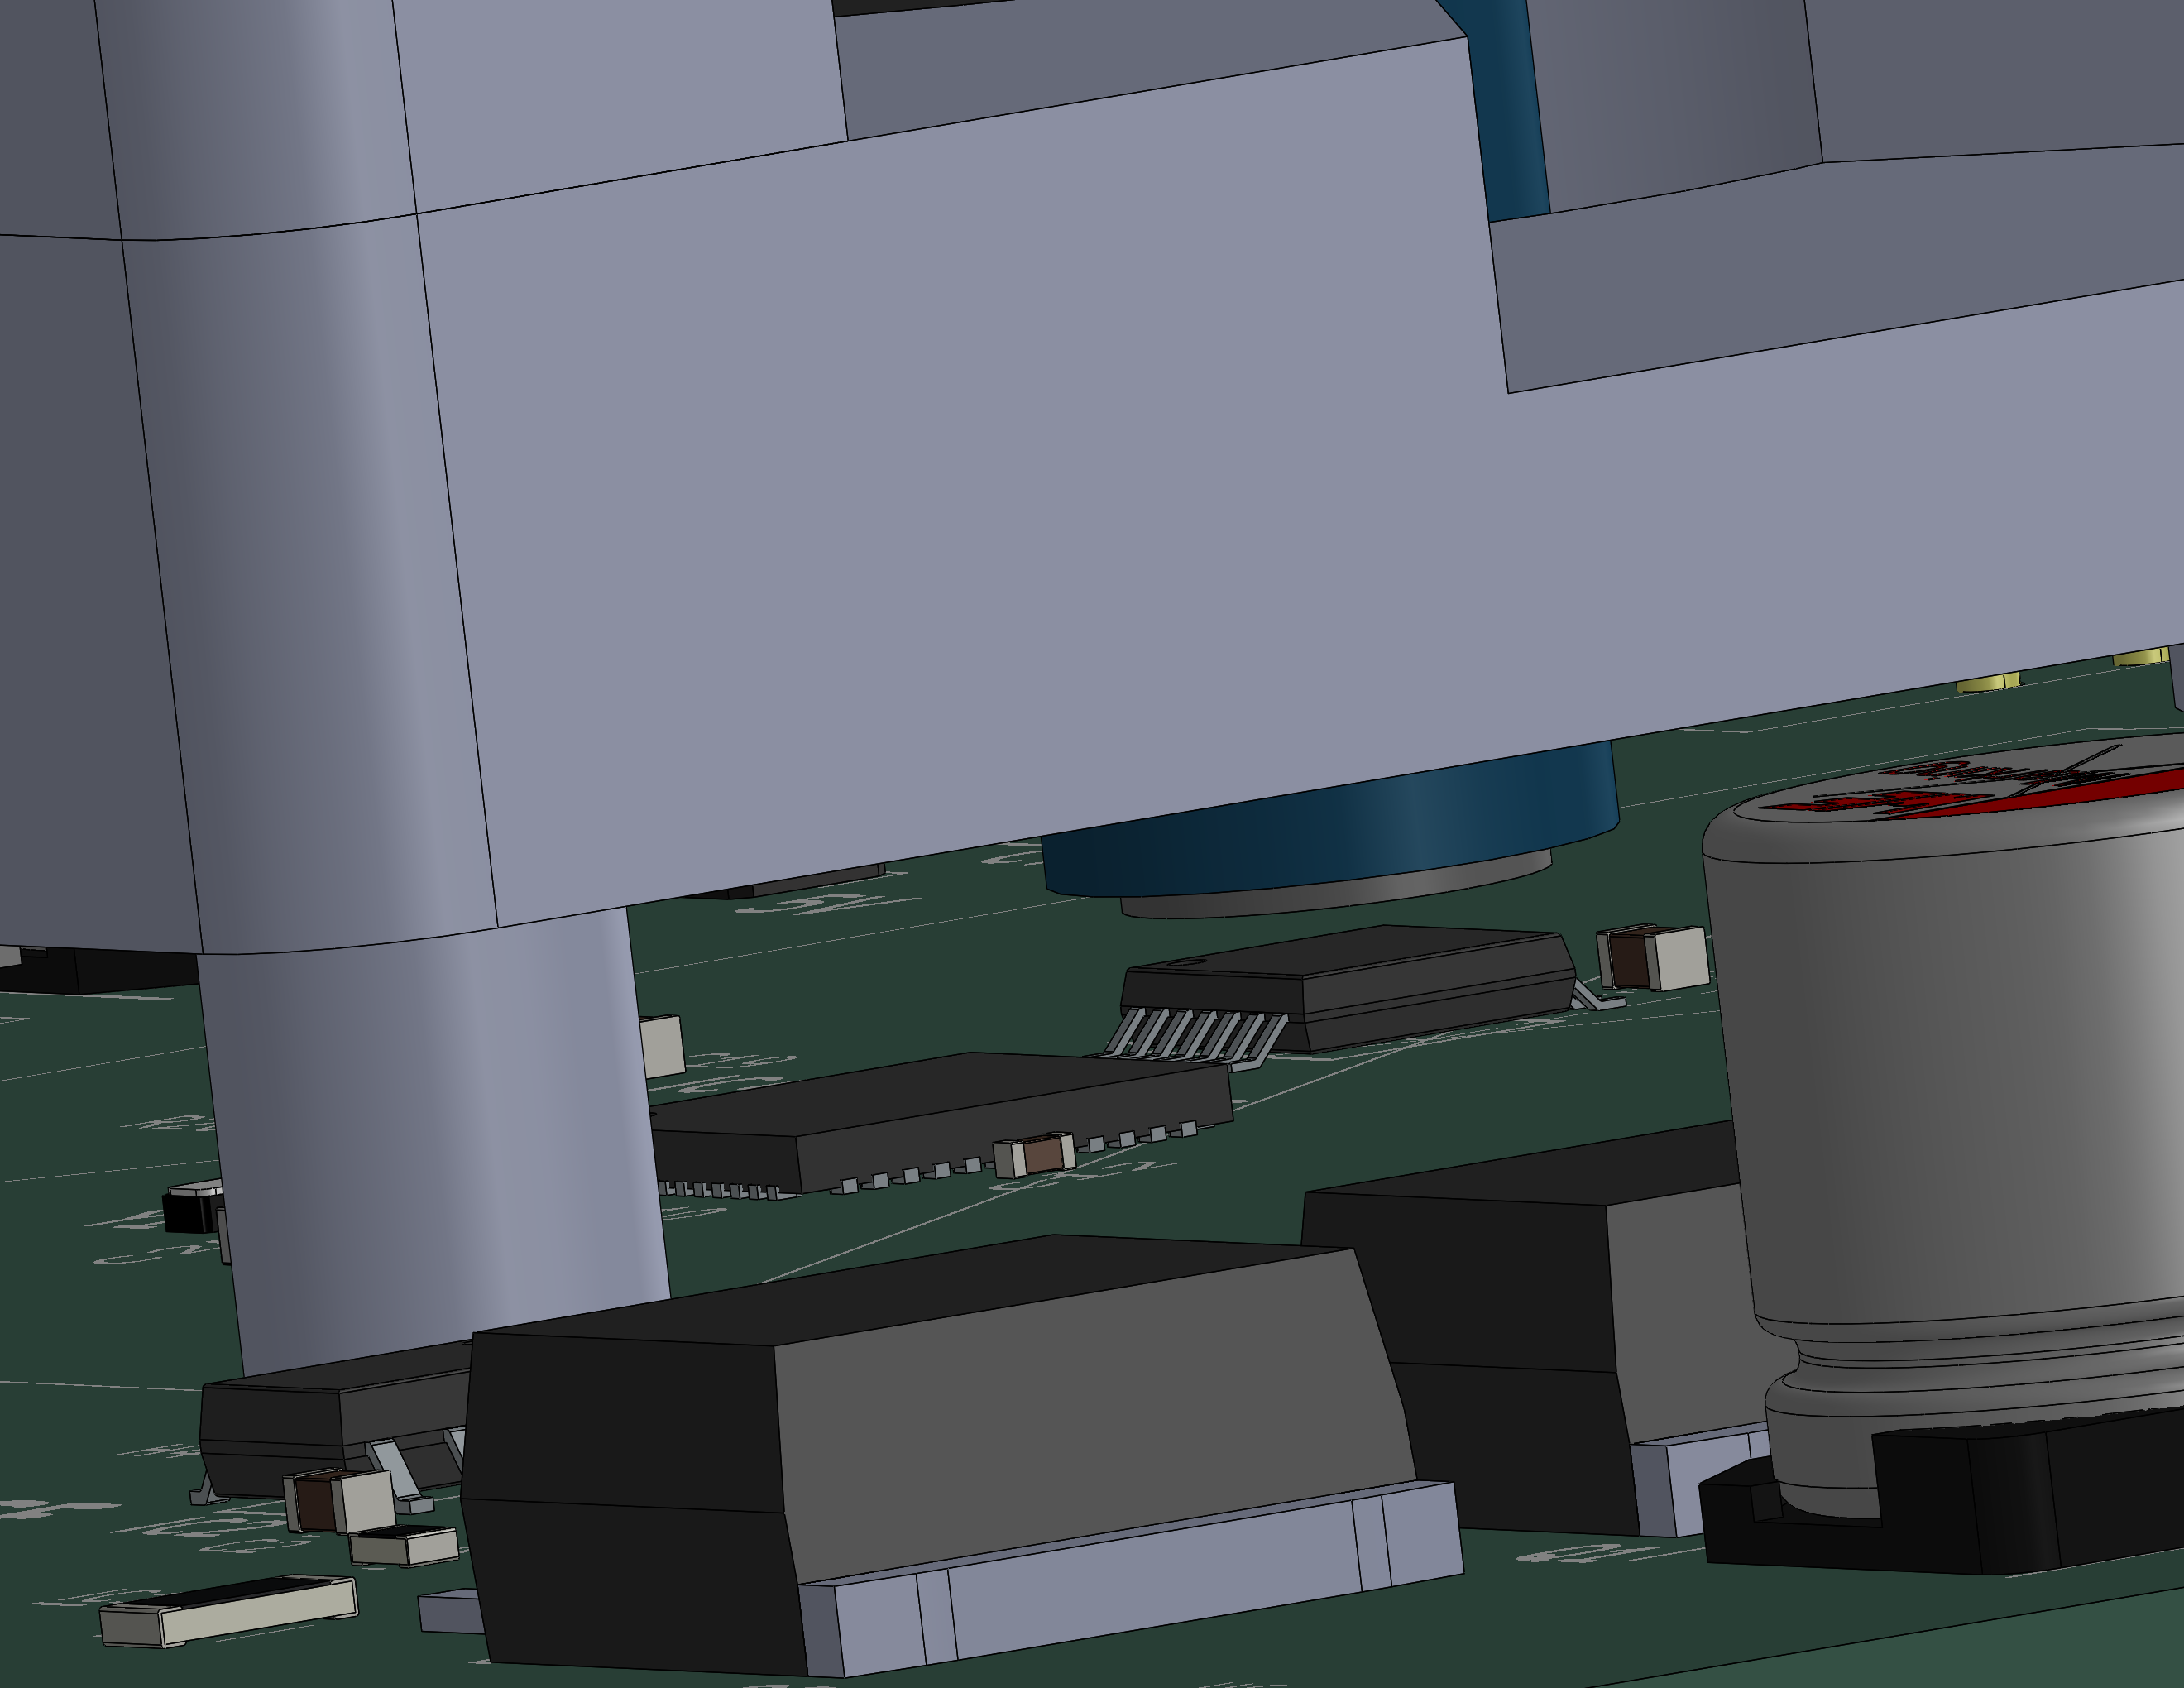
\includegraphics[width=\textwidth, keepaspectratio]{05_SystemLevelTestBench/images/Resolver-PCB-Setup-2.PNG}
        \caption{3D view zoomed to the magnet-encoder alignment}
        \label{fig:assembly-magnet-alignment-zoomed}
    \end{subfigure}

    \caption{Complete mechanical assembly with focus on magnetic encoder to magnet alignment}
    \label{fig:assembly-magnet-alignment}
\end{figure}

As can be seen from the figure \ref{fig:assembly-magnet-alignment}, the blue colored adapter is designed in order to pass through the hollow shaft of the motor and hold the magnet (grey colored on the bottom) on one side and mount the resolver rotor on the other.

In order to make even clearer the alignment and the design internally, in the following figures the supporting structures that hold the components are suppressed in SOLIDWORKS and the placement of the critical components is shown clearly.

\begin{figure}[H]
    \centering
    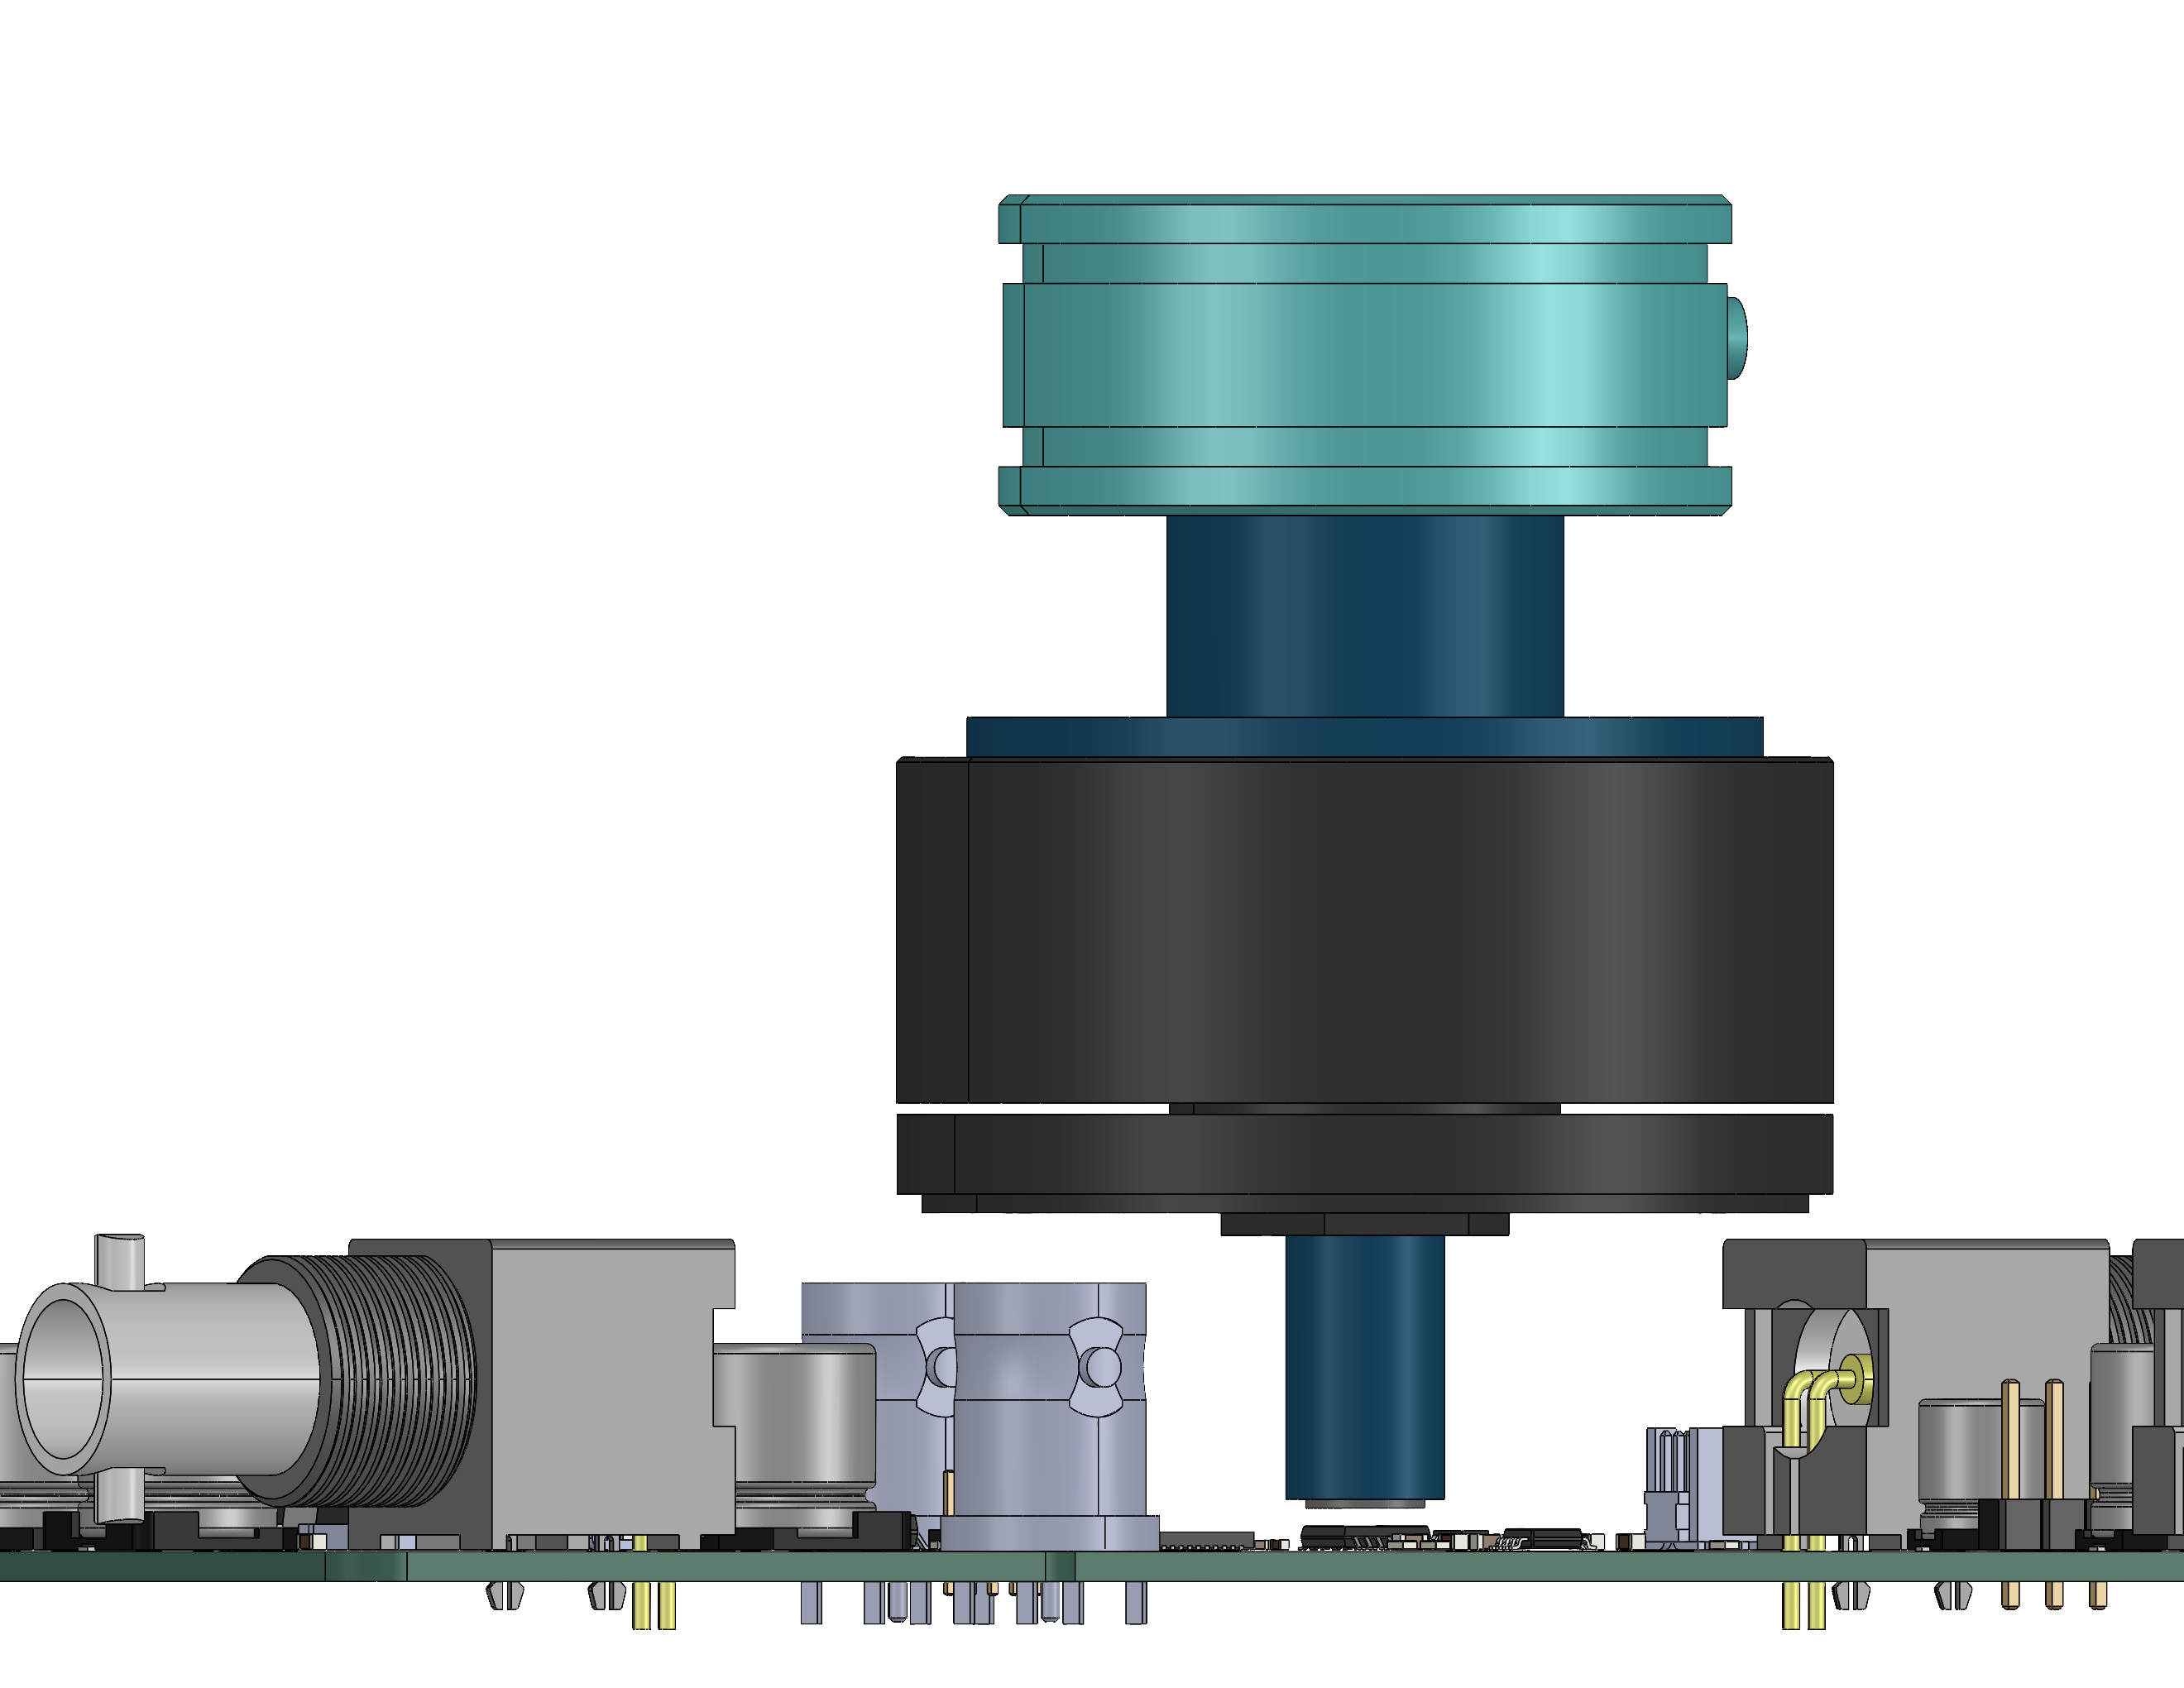
\includegraphics[width=0.6\textwidth, keepaspectratio]{05_SystemLevelTestBench/images/Resolver-PCB-Setup-6.PNG}
    \caption{3D view of the complete mechanical assembly and the PCB of the second iteration system [\ref{subsec:pcb-iter-2}]}
    \label{fig:assembly-panoramic}
\end{figure}

\begin{figure}[H]
    \centering

    \begin{subfigure}[b]{0.48\textwidth}
        \centering
        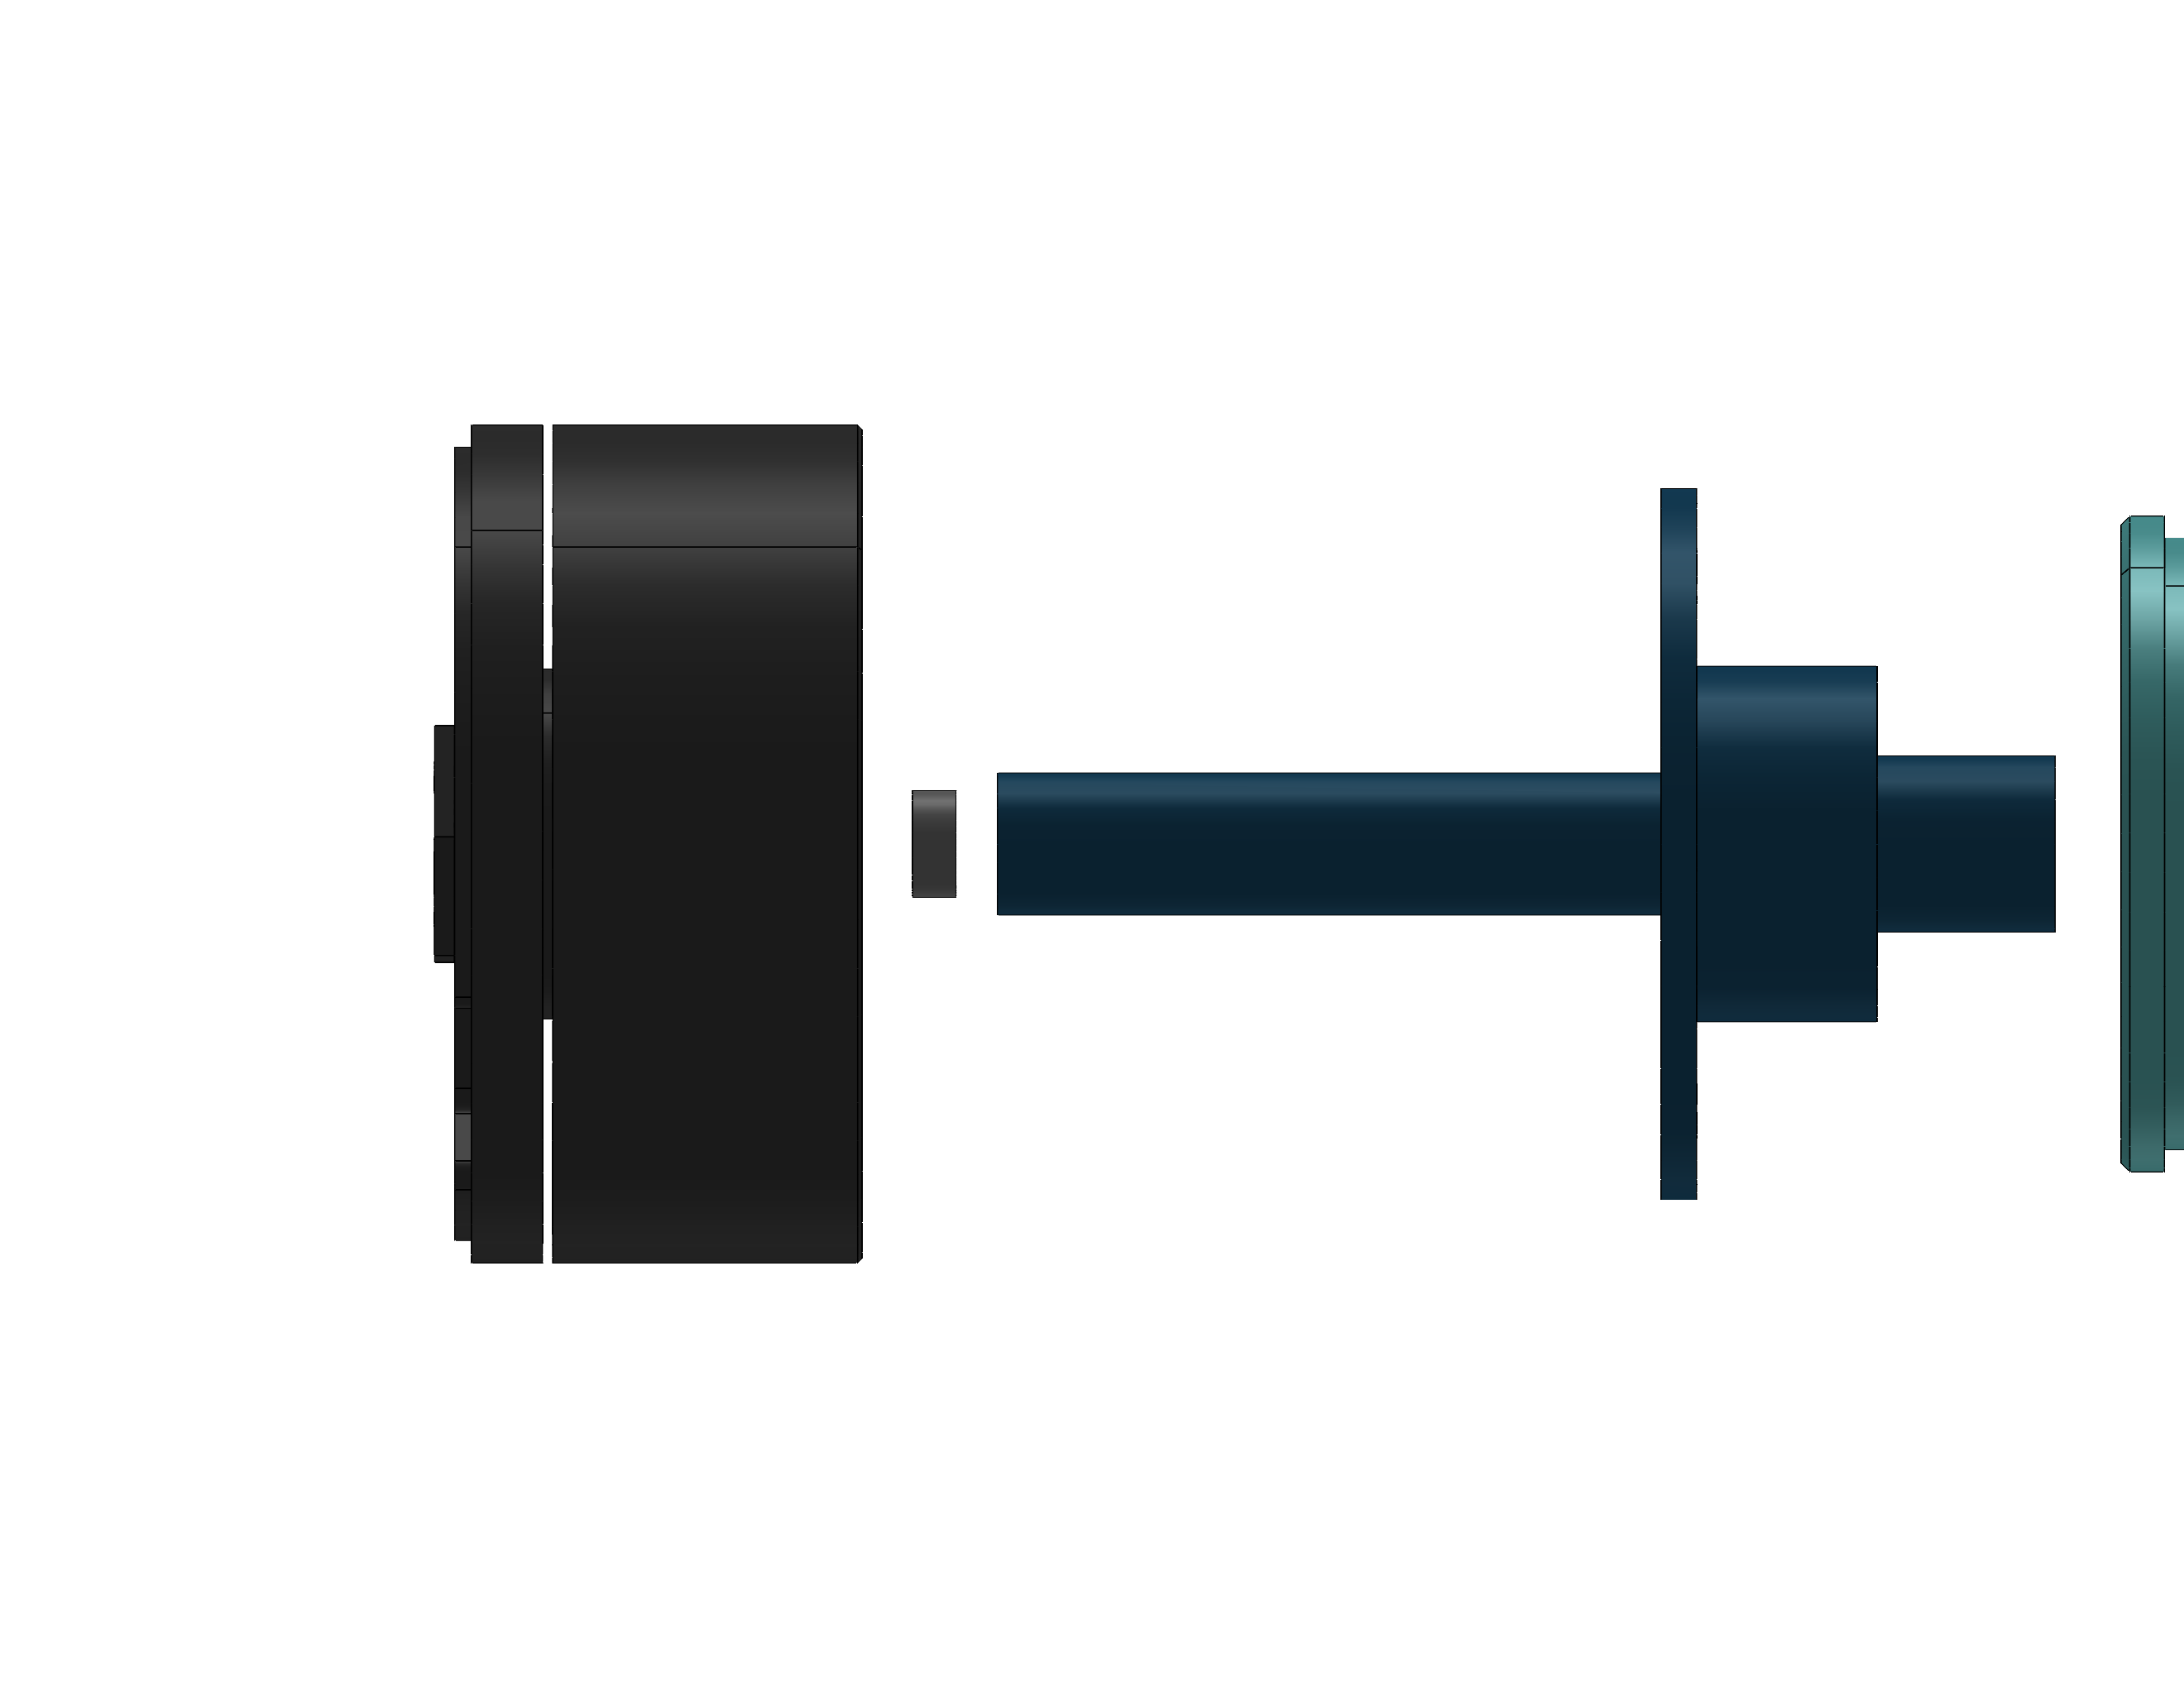
\includegraphics[width=\textwidth, keepaspectratio]{05_SystemLevelTestBench/images/Resolver-PCB-Setup-7.PNG}
        \caption{3D view of the complete mechanical assembly}
        \label{fig:assembly-magnet-alignment-panoramic}
    \end{subfigure}
    \hfill
    \begin{subfigure}[b]{0.48\textwidth}
        \centering
        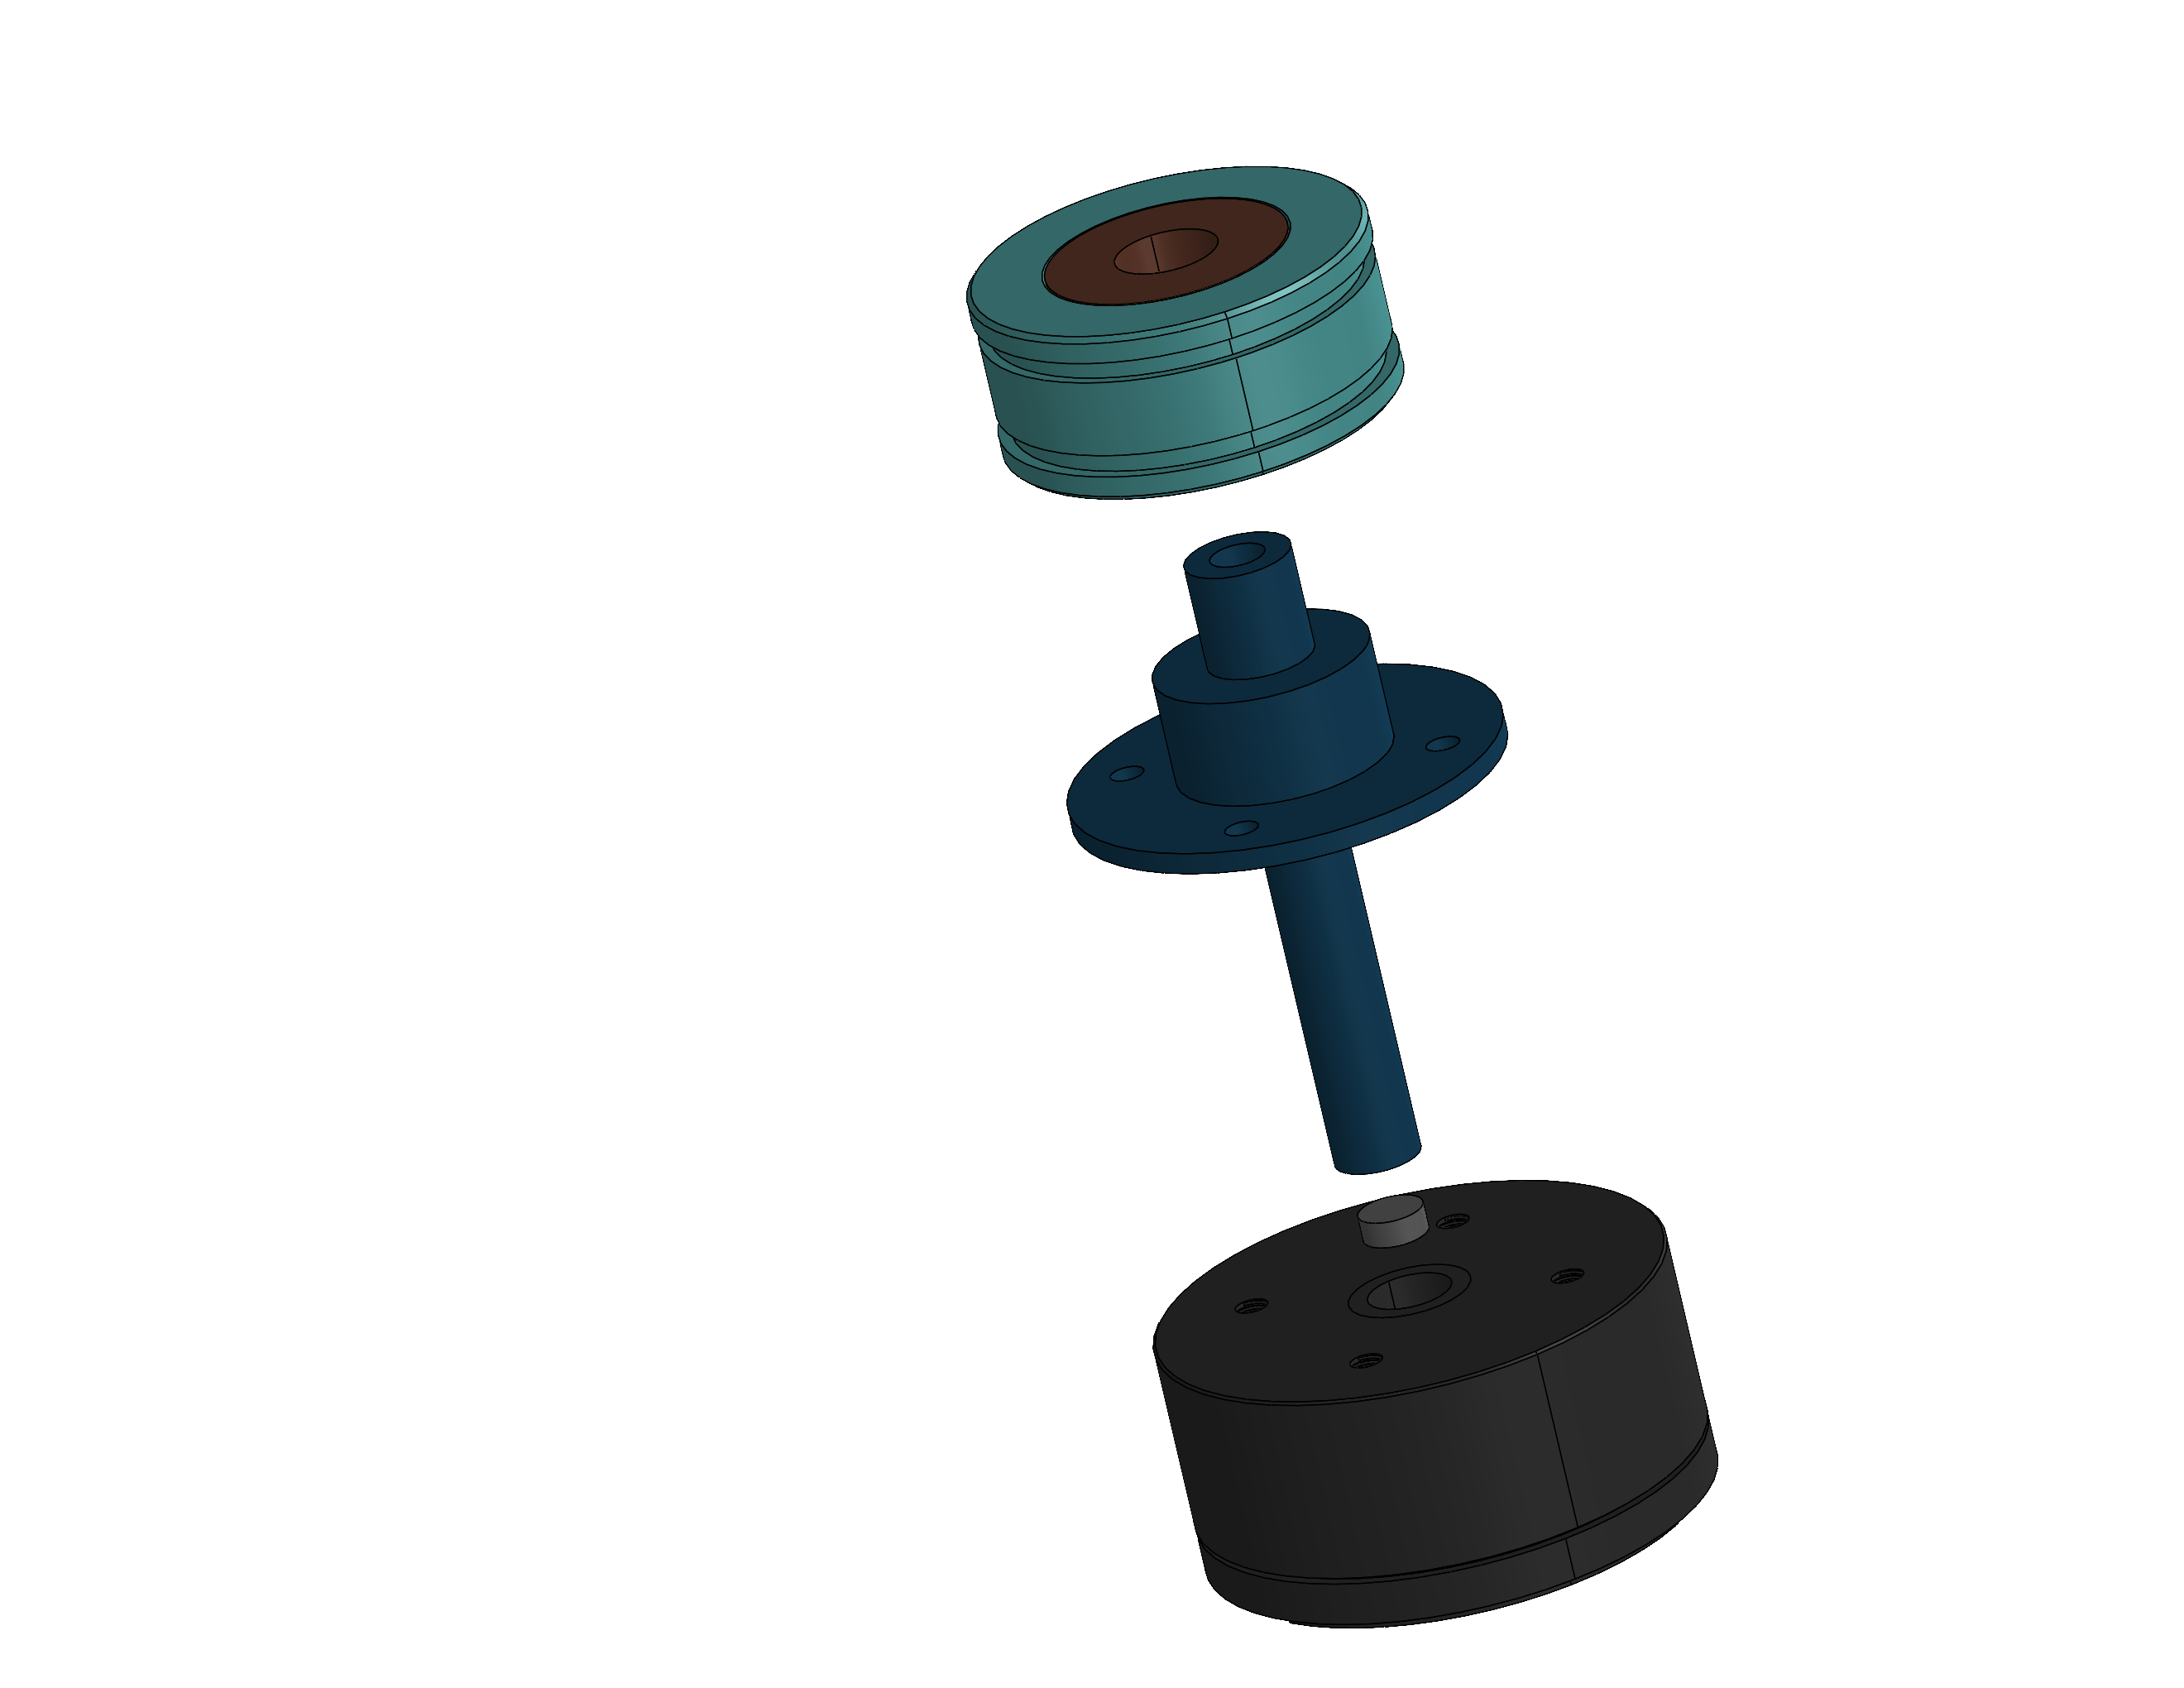
\includegraphics[width=\textwidth, keepaspectratio]{05_SystemLevelTestBench/images/Resolver-PCB-Setup-8.PNG}
        \caption{3D view zoomed to the magnet-encoder alignment}
        \label{fig:assembly-magnet-alignment-zoomed}
    \end{subfigure}

    \caption{Complete mechanical assembly with focus on magnetic encoder to magnet alignment}
    \label{fig:assembly-magnet-alignment}
\end{figure}

\subsection{Material Selection and Manufacturing}
\label{subsec:manufacturing}
The primary manufacturing method used was FDM 3D printing in ABS, chosen for its thermal resistance during motor fault conditions. Since the structure must be reproduced after each CHARM test campaign — as irradiated components cannot be handled or reused outside the irradiation room — disposable 3D-printed parts were the most practical solution.

A version was also machined internally at CERN in aluminium via CNC. Despite the tighter tolerances, the resolver rotor still exhibited slight off-axis rotation, suggesting inherent angular runout in the motor rotor itself rather than a manufacturing deficiency.

Aluminium is non-magnetic, which is critical to avoid distorting the field of the permanent magnet and degrading encoder accuracy. It also simplified grounding, as the structure was bonded directly to board ground at a single point, avoiding ground loops.

\subsection{Resolver Cabling}
\label{subsec:resolver-cabling}

As introduced in Section~\ref{subsec:resolver-readout}, the resolver signals must be routed as twisted pairs. Since dedicated twisted pair cables were not available in the facility, two alternatives were considered:

\begin{itemize}
\item Six individual 50\,$\Omega$ coaxial cables, with signal on the center conductor and the shield as ground reference, or
\item Standard RJ45 Ethernet cables, which contain twisted pairs internally by design.
\end{itemize}

The RJ45 solution was selected. As already motivated in Section~\ref{subsec:facility-constraints}, Ethernet cables and RJ45 patch panels are part of the standard infrastructure at all three facilities, making this choice naturally consistent with the broader connectivity strategy. Beyond signal integrity, this approach is easy to reproduce, straightforward to standardise, and significantly simpler to install than running individual coaxial cables through the facility patch panels.

Therefore, a Telegärtner MFP8-IE Cat.6\textsubscript{A} T568B RJ45 connector~\cite{telegaertner_mfp8_ie_t568b} was mounted at the resolver cable's end.

\subsection{Fully Assembled System Demonstration}
\label{subsubsection:fully-assembled-system}

In figure \ref{fig:full-assembly-lab} is presented the fully assembled setup with all of its components. In chapter \ref{chapter:rad-tests-results} and section \ref{}, the RJ45 is also visible.

\begin{figure}[H]
    \centering
    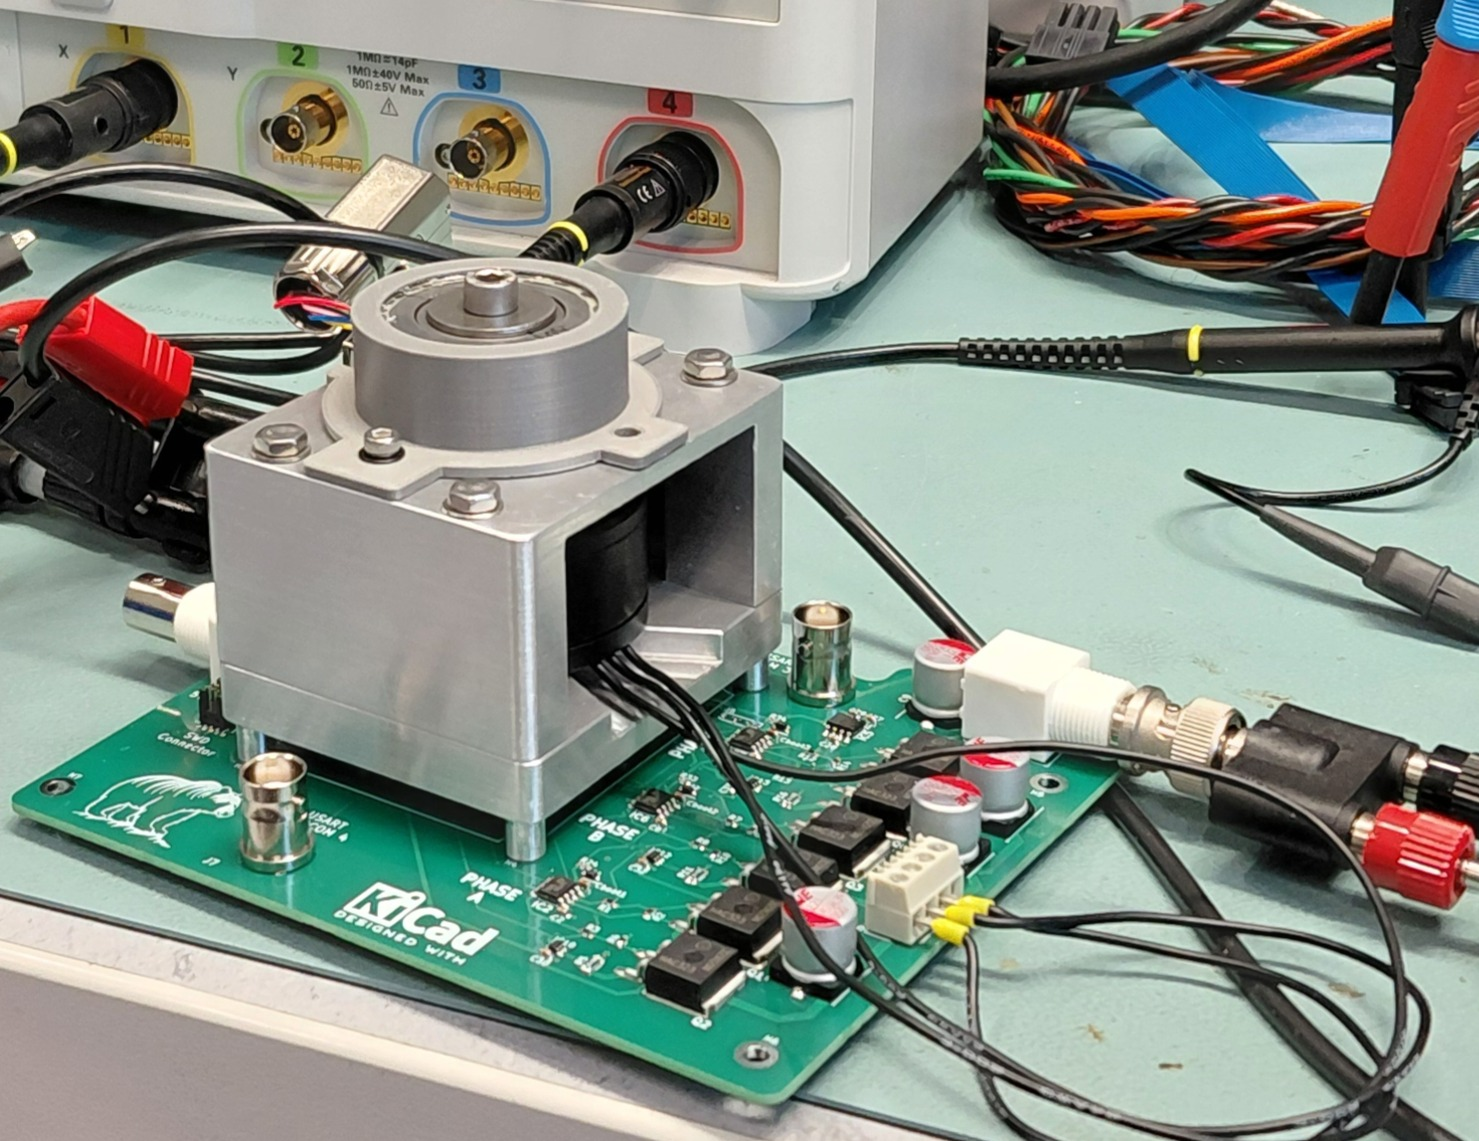
\includegraphics[width=0.6\textwidth, keepaspectratio]{05_SystemLevelTestBench/images/Photo_Assembly_Lab_Cropped.JPG}
    \caption{The fully assembled setup at lab during testing in ambient conditions}
    \label{fig:full-assembly-lab}
\end{figure}

\section{Control Room Software}
\label{section:control-room-sw}

The last piece of the complete test bench setup is the software running in the control room. The software collects all the signals from the test system, namely the USART channels and the resolver signals. It is implemented in Python and C++.

\begin{figure}[H]
    \centering
    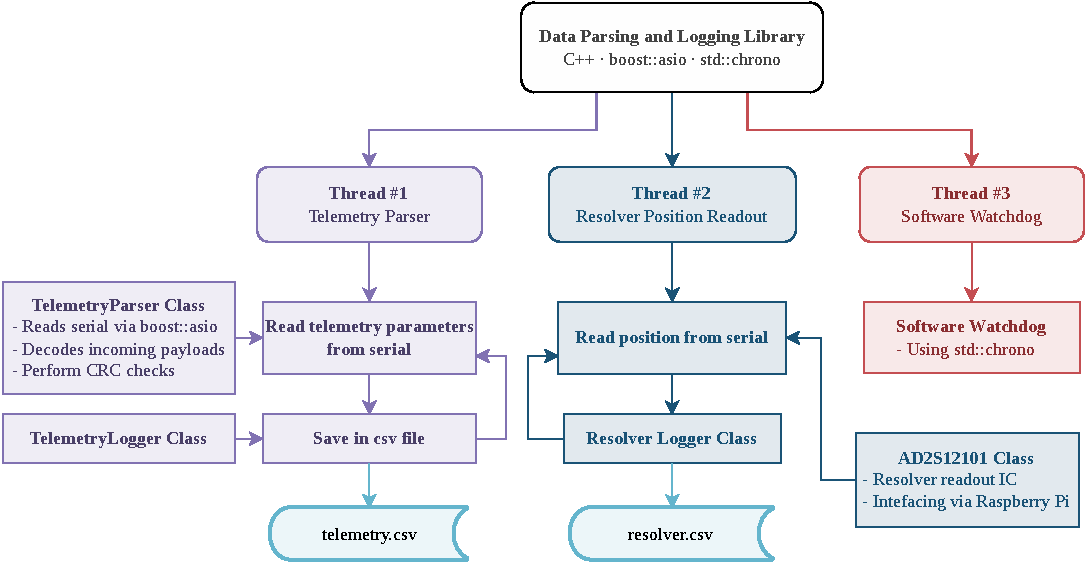
\includegraphics[width=\textwidth, keepaspectratio]{05_SystemLevelTestBench/images/ControlRoomSoftwareOverview_cpp.pdf}
    \caption{The C++ implementation of the acquisition software}
    \label{fig:control-room-software-cpp}
\end{figure}

% The idea behind the software is to create three different threads that run in parallel as infinite loops. The responsibilities of each thread are well defined: the first one reads the incoming telemetry from the serial port using the \texttt{boost::asio} library and decodes the bytes. The decoded information is then logged in a CSV file on the hard disk. The second thread is responsible for reading the position from the independent resolver. A lightweight C++ driver, based on an existing repository script, reads the angle from the resolver and stores it in a CSV file on the hard drive. The resolver should be sampled at the highest safe frequency, as it is intended to serve as the primary data source for analysis. A third thread implements a software watchdog, providing this functionality on system variants that lack an external hardware watchdog by triggering a power cycle.

The software runs three parallel threads, each implemented as an infinite loop, with clearly defined responsibilities. The first reads and decodes incoming telemetry from the serial port using the \texttt{boost::asio} library, logging the result to a CSV file on disk. The second reads the position from the independent resolver through a lightweight C++ driver, based on an existing repository script, and stores the angle in a CSV file; since the resolver serves as the primary data source for analysis, it is sampled at the highest safe frequency. A third thread implements a software watchdog, providing this functionality on system variants that lack an external hardware watchdog by triggering a power cycle.

The watchdog monitors two events, summarized in Table~\ref{tab:software-watchdog}, and triggers a power cycle in response to either.

\begin{table}[H]
    \centering
    \arrayrulecolor{thesisblue}
    \renewcommand{\arraystretch}{1.25}
    \setlength{\tabcolsep}{8pt}
    \begin{tabular}{
        >{\centering\arraybackslash}m{3.0cm}
        >{\centering\arraybackslash}m{5.2cm}
        >{\centering\arraybackslash}m{4.5cm}
    }
        \rowcolor{thesisblue}
        \textcolor{white}{\textbf{Event}} &
        \textcolor{white}{\textbf{Condition}} &
        \textcolor{white}{\textbf{Watchdog Action}} \\
        \hline
        \rowcolor{thesislightgray}
        Resolver angle unchanged &
        Persists for $>$2 minutes &
        Log timeout, trigger power cycle \\
        No incoming UART data &
        No data for $>$20 s (possible MCU crash) &
        Log timeout, trigger power cycle \\
        \hline
    \end{tabular}
    \caption{Watchdog-monitored events and their corresponding actions.}
    \label{tab:software-watchdog}
    \arrayrulecolor{black}
\end{table}

The software is compiled and launched by the PSU control Python script, which runs it as a sub-process. This script is the highest-level script executed in the terminal and serves a dual purpose: sampling the PSUs via PyVISA and SCPI commands to periodically read the currents and log them to a CSV file along with a Unix timestamp, and power cycling the DUT in the event of a fault. The important point here is that fault detection occurs in the C++ software and is communicated to the Python script, which then triggers a power cycle. The C++ software writes the resolver positions to stderr, which the Python script reads via a dedicated thread and prints to the console. A second thread reads from stdout, where the C++ code writes machine-readable commands, causing the Python script to trigger a power cycle upon receiving a fault notification.
The whole thing is presented in figure \ref{fig:control-room-software}.

\begin{figure}[H]
    \centering
    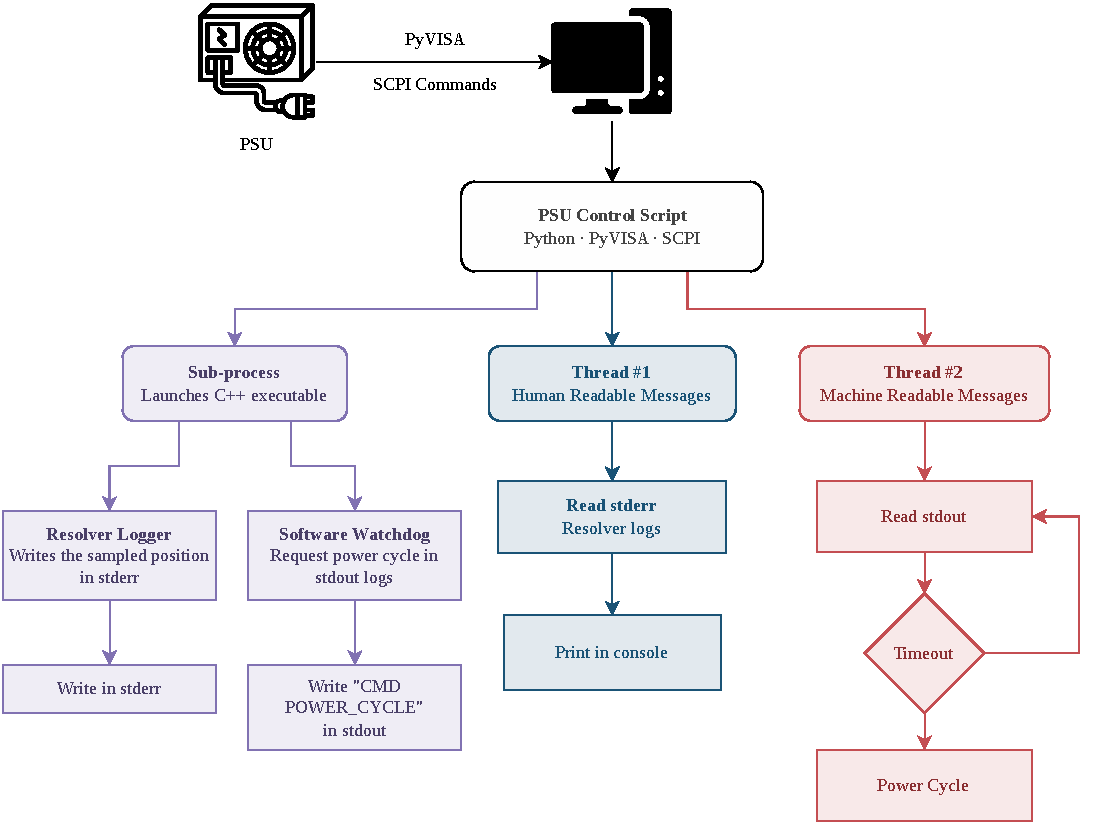
\includegraphics[width=\textwidth, keepaspectratio]{05_SystemLevelTestBench/images/ControlRoomSoftwareOverview.pdf}
    \caption{The complete data acquisition software business logic.}
    \label{fig:control-room-software}
\end{figure}

\section{Data Acquisition and Analysis Methodology}
\label{sec:data-acquisition-methodology}

\subsection{Initial Test Data Post-Processing}
\label{subsection:data-post-processing}

As discussed in Section~\ref{section:control-room-sw}, the data are stored as raw in a csv format file, therefore a some processing is required in order to be in a useful form for making conclusions.

\subsubsection*{Dosimetry Acquisition in Different Facilities}

The big difference between CHARM and the PSI and CC60 facilities is that the dose rate at CHARM is nowhere near constant. Thus, the facility's dosimetry service provides the dosimetry data for CHARM during the various irradiation weeks. On the other hand, the dose rate is stable in PSI and CC60, and for that reason, the first step of the analysis is to convert the time into accumulated ionizing dose and, where relevant, displacement damage equivalent fluence.

Supposing that $t_0$ is the starting time of irradiation, the total elapsed time (given in hours) till $t_i$ since the irradiation started is

\begin{equation*}
    \Delta t_i = \frac{t_i-t_0}{3600}
\end{equation*}

Furthermore, since the dose rate is stable, $\dot{D} = \frac{dD}{dt}$, the corresponding TID is then given by the formula,

\begin{equation*}
    TID_i = \dot{D} \cdot \Delta t_i
\end{equation*}

At CC60, TID is the only quantity of interest since the photon field produces negligible displacement damage compared to the ionizing dose. At PSI, displacement damage is also of interest and expressed as the 1MeV-DDEF~\cite{ferraro_phd_thesis}. Since the beam delivers a stable dose rate, DDEF accumulates proportionally to TID, given by the following equation.

\begin{equation*}
    DDEF_i = 1.69\times10^{9}~\text{cm}^{-2}\,\text{Gy}^{-1} \cdot TID_i.
\end{equation*}

\subsection{Position Samples Characterization}
\label{subsection:position-samples-characterization}
As discussed throughout this chapter, two sensors are used to sample the rotor position: the magnetic encoder and the golden-reference resolver. Since the AS5047P provides the angle as a 14-bit raw value, it must be converted to degrees as
\begin{equation*}
    \theta\,[^\circ] = \frac{360^\circ}{2^{14}} \cdot \theta_{raw}.
\end{equation*}
Furthermore, since the motion is circular and periodic, crossing the $0^\circ/360^\circ$ boundary requires attention, as it introduces large spikes when computing the speed through the differentiation $\omega = d\theta/dt$, or, in its discrete form obtained via finite differences,
\begin{equation*}
    \omega_i \approx \frac{\theta_{i+1} - \theta_{i-1}}{t_{i+1} - t_{i-1}}.
\end{equation*}
For this reason, the unwrapped angle $\theta^{\text{unwrapped}}$ is used instead, so that the expression becomes
\begin{equation*}
    \omega_i \approx \left|\frac{\theta^{\text{unwrapped}}_{i+1} - \theta^{\text{unwrapped}}_{i-1}}{t_{i+1} - t_{i-1}}\right|.
\end{equation*}
The direction of rotation is not relevant here and is therefore disregarded. The purpose of computing the speed is to classify each sample into one of two categories: \textit{i) transient}, and \textit{ii) settled}. This distinction matters because only the settled samples are used to evaluate accuracy and repeatability.

Moreover, differentiation creates another problem: it makes the calculation highly sensitive to sampling noise. As a result, the angular velocity has to be smoothed before it can be used. For this, a rolling-median filter is used, since it is less sensitive to isolated spikes than a moving-average filter.

The filtered angular speed, denoted $\widetilde{\omega}_i$, is then classified using two separate thresholds: $h_{\mathrm{transient}}$, crossed while the rotor is accelerating, and $h_{\mathrm{settled}}$, crossed while the rotor is decelerating toward zero, which signals that the motion has settled. Mathematically, this is captured by the rule
\begin{equation*}
    f_i = \begin{cases}
        1, & \widetilde{\omega}_i \geq h_{\mathrm{transient}}, \\
        0, & \widetilde{\omega}_i \leq h_{\mathrm{settled}}, \\
        f_{i-1}, & h_{\mathrm{settled}} < \widetilde{\omega}_i < h_{\mathrm{transient}},
    \end{cases}
\end{equation*}
where $f_i = 1$ marks a moving sample and $f_i = 0$ marks a settled one. The third line is what makes the rule work: whenever the filtered speed falls between the two thresholds, the sample simply keeps the same label as the one before it, instead of switching back and forth every time the speed jitters slightly.

Finally, the samples $i$ that map to $f_i = 0$ are kept for the analysis in terms of accuracy and repeatability of the control system.

\subsection{Accuracy and Repeatability Metrics}
\label{subsec:accuracy-repeatability-metrics}

\subsubsection*{Definitions}
Accuracy and repeatability are two core evaluation parameters when benchmarking a control system. While they might seem similar, they correspond to different properties of the system.

\textbf{Accuracy} is the ability of the system to reach a final position close to the commanded position. In other words, it is a measure of the difference between the user commanded target (input in software) and the physical settling of the rotor (hardware output)~\cite{motionsolutions_accuracy_misconceptions}.

\textbf{Repeatability} is the ability of the system to reach the same actual position consistently under repeated identical commands. It is often considered one of the most critical metrics in robotics, since poor accuracy can in principle be corrected in software once it has been characterized, whereas poor repeatability cannot be compensated for in the same way~\cite{motionsolutions_accuracy_misconceptions}.

A visual reference for both metrics is provided in Figure~\ref{fig:accuracy-repeatability}.

\begin{figure}[H]
\centering
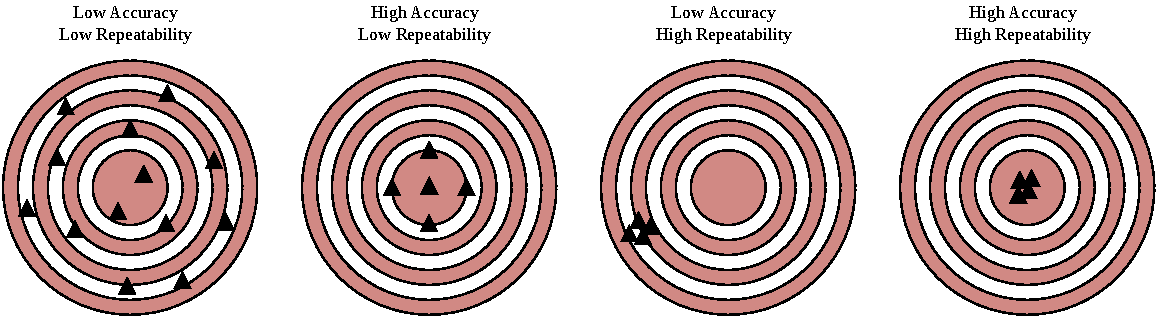
\includegraphics[width=\textwidth,keepaspectratio]{05_SystemLevelTestBench/images/Accuracy_Repeatability.pdf}
\caption{Illustration of accuracy and repeatability and their distinction for a positioning system.}
\label{fig:accuracy-repeatability}
\end{figure}

Both the encoder angle (from the telemetry UART, used directly by the control algorithm) and the independent resolver angle are used to evaluate these metrics. However, before any comparison is attempted, the constant zero-reference offset between the two sensors must be isolated, since the encoder and resolver do not share the same zero angle. This offset is illustrated in Figure~\ref{fig:encoder-resolver-offset}.

\begin{figure}[H]
\centering
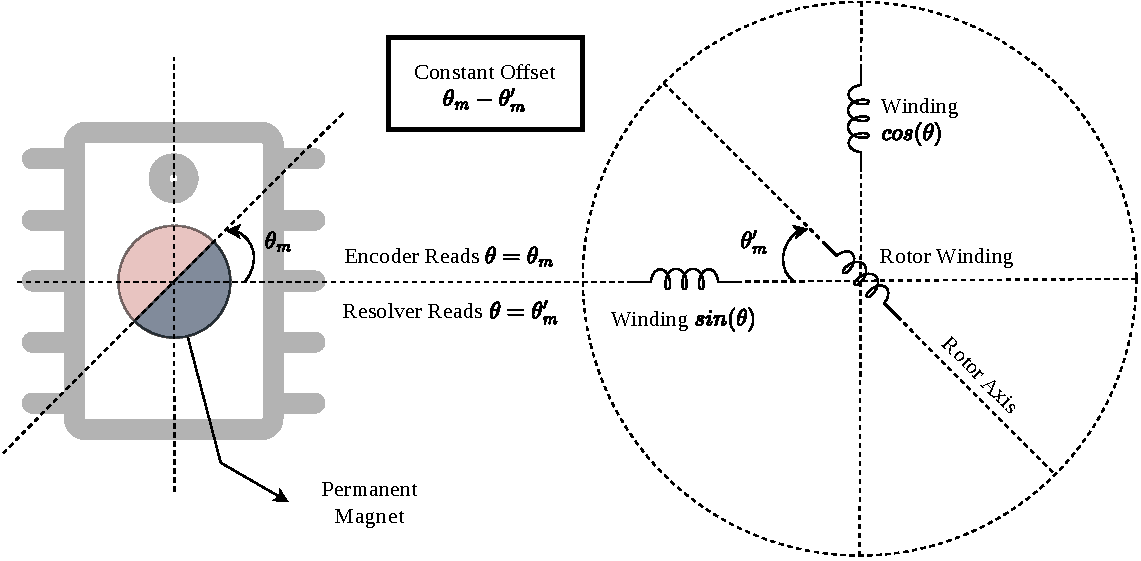
\includegraphics[width=\textwidth,keepaspectratio]{05_SystemLevelTestBench/images/Encoder_Resolver_Offset.pdf}
\caption{The constant angular offset between encoder and resolver readings due to their different interpretation of $0^\circ$.}
\label{fig:encoder-resolver-offset}
\end{figure}

In practice, the encoder angle represents the accuracy of the closed-loop controller, since it is the quantity the firmware attempts to drive to the commanded value. The resolver provides an independent ground truth to validate those results. Repeatability is derived from the resolver data rather than the encoder, since the encoder is part of the DUT while resolver is the trustworthy golden reference.

\subsubsection*{Commanded Angles and Quantization Error Derivation}

The demo that runs during radiation tests is set to drive the rotor to four absolute target angles, issued in firmware in mrad,

\begin{equation*}
    c_k \in \{0,\,1571,\,3141,\,4712\}~\si{\milli\radian}, \qquad k = 0,1,2,3.
\end{equation*}

Because the targets are absolute rather than incremental, the positioning error does not accumulate from cycle to cycle. Converting to degrees,

\begin{equation*}
    \theta_{\mathrm{cmd}}^{(k)} = \frac{180^\circ}{\pi}\,\frac{c_k}{1000},
\end{equation*}

gives a command resolution of $1~\si{\milli\radian} = 0.0573^\circ$. Therefore, the real target angles that the encoder accepts are $0^\circ$, $90.012^\circ$, $179.966^\circ$ and $269.978^\circ$.

This command-level quantization is independent of the quantization introduced by the encoder's own 14-bit raw output, discussed in Subsection~\ref{subsec:expected-accuracy-repeatability}, which instead limits the resolution at which the settled rotor position can be read back rather than the resolution of the commanded target.

\subsection{Estimated Sensor Accuracy and Repeatability}
\label{subsec:expected-accuracy-repeatability}
Before making any claims on the accuracy and repeatability results of the tests, it is important to determine the baseline accuracy the sensor can deliver independently of any radiation effect. The relevant accuracy-related parameters reported in the sensor's datasheet~\cite{as5047p_datasheet} are summarized in Table~\ref{tab:as5047p-specs}.

\begin{table}[H]
    \centering
    \arrayrulecolor{thesisblue}
    \renewcommand{\arraystretch}{1.25}
    \setlength{\tabcolsep}{8pt}
    \begin{tabular}{
        >{\centering\arraybackslash}m{7.5cm}
        >{\centering\arraybackslash}m{4.5cm}
    }
        \rowcolor{thesisblue}
        \textcolor{white}{\textbf{Parameter}} &
        \textcolor{white}{\textbf{Value}} \\
        \hline
        \rowcolor{thesislightgray}
        Core resolution (SPI) &
        \SI{14}{bit} \\
        Quantization noise (RMS), \cite{kester_mt001} &
        \SI{0.0063}{\degree} \\
        \rowcolor{thesislightgray}
        Output noise, $1\sigma$ &
        \SI{0.068}{\degree} \\
        INL, optimum placement @\SI{25}{\celsius} &
        $\pm\SI{0.8}{\degree}$ \\
        \rowcolor{thesislightgray}
        INL, optimum placement, full temp. &
        $\pm\SI{1.0}{\degree}$ \\
        INL, with magnet displacement + temp. &
        $\pm\SI{1.2}{\degree}$ \\
        \rowcolor{thesislightgray}
        Required field strength $B_z$ &
        \SIrange{35}{70}{\milli\tesla} \\
        \hline
    \end{tabular}
    \caption{Factors that affect the accuracy of the AS5047P.}
    \label{tab:as5047p-specs}
    \arrayrulecolor{black}
\end{table}

Of these, accuracy is bounded by the non-linearity terms (INL), since they represent a systematic, repeatable bias, while repeatability is bounded by the output-noise term, since it reflects random sample-to-sample scatter rather than a fixed offset. Note that for many encoders, repeatability is not given as a separate specification and is instead folded into a single accuracy figure~\cite{rls_encoder_handbook}. The AS5047P datasheet is more granular in this respect, reporting non-linearity and output noise as two distinct parameters, which is what makes it possible to budget the two metrics separately in what follows.

INL captures the angular error introduced by imperfect alignment between the magnet and the IC, and is the dominant contributor to the accuracy budget, roughly an order of magnitude larger than either the quantization or output-noise terms~\cite{as5047p_datasheet} (note that ams's product overview separately quotes a typical, condition-unspecified accuracy of \SI{0.5}{\degree}~\cite{as5047p_product_page}, which is not directly comparable to the worst-case INL bound used here). Since the magnet holder is produced by 3D printing or CNC machining, dimensional tolerances on the x, y, and z axes introduce an uncontrolled offset between the magnet and the die, placing the relevant figure closer to the displacement case than to the optimum-placement case~\cite{as5047p_datasheet}.

DAEC was enabled throughout all tests; it compensates for the dynamic angle error caused by signal propagation delay at high rotational speed, and since this error is zero at standstill, it has no effect on the settled-position measurements used in this evaluation~\cite{as5047p_daec_appnote}.